\section{Nuværende omkostninger i sundhedssektoren}
Det er relevant at se på omkostningerne i sundhedssektorens primære og sekundære sektor ved brug af den nuværende målemetode. 

\subsection{Primær sektor} \label{sec:nuv_primaer}
Den subjektive målemetode, der på nuværende tidspunkt benyttes af $27,7~\%$ af praktiserende læger, foregår ved spørgeskema under en konsultation, medfører udgifter i den primære sundhedssektor \citep{munck2007}. Afhængigt af antal konsultationer, som den enkelte kronikere har behov for, kan et spørgeskema følge med hver konsultation, og omkostningerne til denne målemetode vil derved stige. Udarbejdelse og udskrifter af et spørgeskema vil have relativt lave omkostninger.
\citeauthor{munck2007} udarbejdede i 2007 en rapport om hypertension i almen praksis. Her blev $159$ kontaktpersoner i almen praksis spurgt: "Sætter I jeres hypertensionspatienter til kontrol med fast tidsinterval? Hvis ja, angiv det typiske interval". Her svarede $92,5~\%$, at de sætter deres patienter til kontrol med et fast tidsinterval, og i gennemsnit er dette interval udregnet til $3,9$ måneder \citep{munck2007}. 

Hvis det, jævnfør \citeauthor{kronborg2008}, antages at $1/5$ af den voksne danske befolkning har hypertension, vil dette svare til omkring $900.000$ danskere \citep{folketal2016}. Hvis $900.000$ danskere skal til lægekonsultation á $137,93$ kroner hver $3,9$. måned, vil dette svare til en årsomkostning for sundhedssektoren på omkring $380$ millioner kroner \citep{honorartabel2016}. 

Den samlede medicinudgift i den primære sundhedssektor i Danmark i $2014$ lå på $11,6$ milliarder kroner, og Danmarks Statistik påpeger i denne sammenhæng, at blodtrykssænkende medicin og hjertemedicin er nogle af de mest anvendte former for medicin i Danmark \citep{dst2016}. 

Ifølge rapporten "Lægemidler i Danmark 2012" af Danmarks apotekerforening oplyses at det mest udleverede blodtrykssænkende lægemiddeler er amlodipin (139 DDD), furosemid (94 DDD), ramipril (92 DDD), bendroflumenthiazid og kalium (85 DDD), enalapril (80 DDD), samt losartan (73 DDD). I år 2012 blev der udleveret hvad der svarer til 563 millioner døgndoser (DDD) af disse lægemiddel for hele den danske befolkning \citep{apotekerforeningen2012}. Hvis aktivitetsarmbånd som en non-farmakologisk  behandling vil der kunne spares på DDD for patienter med hypertension hvis denne metode kan påvirke patienternes helbred positivt. Ud over besparelser på DDD vil bivirkninger ved lægemidlerne også kunne reduceres, hvilket vil resultere i bedre livskvalitet for patienterne, samt et lettere behandlingsforløb. Eksempler på de hyppigste bivirkningerne ved de fleste af de nævnte lægemidler er, ødemer, dehydrering, træthed, hovedpine og svimmelhed. Den bedste medicinering mod hypertension er individuel, hvorfor det ofte er nødvendigt at finde de lægepræparater der er mest effektive for den enkelte patient, uden at der er for mange bivirkninger.  

%\textbf{+ Tilføj evt. noget omkring definerede døgndoser ud fra \url{pro.medicin.dk}, hvor der står priser på forskellige præparater, og ifølge \citeauthor{munck2007}, hvor der står procenttal på, hvad de hypertensive patienter bruger af medicin. }

\subsection{Sekundær sektor}
Den sekundære sektor påvirkes også af hypertension på den måde, at sygdommen er skyld i ambulante besøg og indlæggelser. I $2014$ var der $49.875$ ambulante besøg i den offentlige sekundære sektor for patienter med diagnosen blodtryksforhøjelse af ukendt årsag eller blodtryksforhøjelse af kendt årsag, hvilket svarer til en stigning på $8,35~\%$ siden $2012$, hvilket kan ses på \autoref{fig:hyp_sekundaer} \citep{sundhedsdatastyrelsen2016}. 

\begin{figure}[H]
\centering
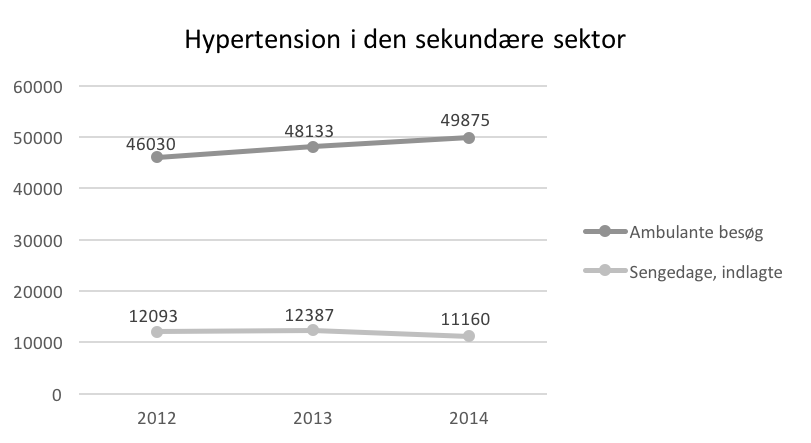
\includegraphics[width=0.8\textwidth]{figures/hyp_sekundaer}
\caption{Henvendelser i den offentlige sekundære sektor som følge af hypertension fra 2012 til 2014 \citep{sundhedsdatastyrelsen2016}.}
\label{fig:hyp_sekundaer}
\end{figure}

\noindent
Yderligere havde patienter med hypertension $11.160$ sengedage i forbindelse med indlæggelse på offentlige sygehuse i $2014$, hvilket var et fald i forholdt til de to foregående år \citep{sundhedsdatastyrelsen2016}. 

Jævnfør \citeauthor{takstvejledning2016} er taksten for et ambulant besøg  med journaloptagelse 1.421 kroner uden nogen særlige procedurer, og taksten for en indlæggelse af en patient med hypertension er $12.597$ kroner indtil fire dage, der er det maksimale antal sengedage, der er dækket af denne takst. Ud over fire dage kan der opkræves en brugerbetaling for langliggertakst på $1.976$ kroner \citep{takstvejledning2016}. 

Hvis det antages, at ambulante besøg og antal sengedage i $2014$ er tilsvarende til henvendelser i år $2016$, så vil prisen for dette være omkring $210$ millioner kroner for ét år. 